\section{24 - MAT - AN 1.1, FA 2.2, FA 5.2, FA 5.3, FA 5.6, WS 1.1, WS 1.2 - Bev�lkerungsentwicklung - BIFIE Aufgabensammlung}

\begin{langesbeispiel} \item[0] %PUNKTE DES BEISPIELS
				Die Weltbev�lkerung ist in den vergangenen Jahrhunderten unterschiedlich stark gewachsen. F�r die weitere Entwicklung bis zum Ende dieses Jahrhunderts gibt es unterschiedliche Prognosen.
				
				Abbildung 1 zeigt die Bev�lkerungsentwicklung in den vergangenen 3\,000 Jahren.\\			
				Abbildung 2 zeigt die Bev�lkerungsentwicklung von 1750 bis 2010.\\				
				Abbildung 3 zeigt die Bev�lkerungsentwicklung von 1950 bis 2010.
				
				Die untenstehende Tabelle zeigt die Bev�lkerungsentwicklung nach Kontinenten und Subkontinenten von 1900 bis 2000.
				
				\begin{center}\resizebox{0.6\linewidth}{!}{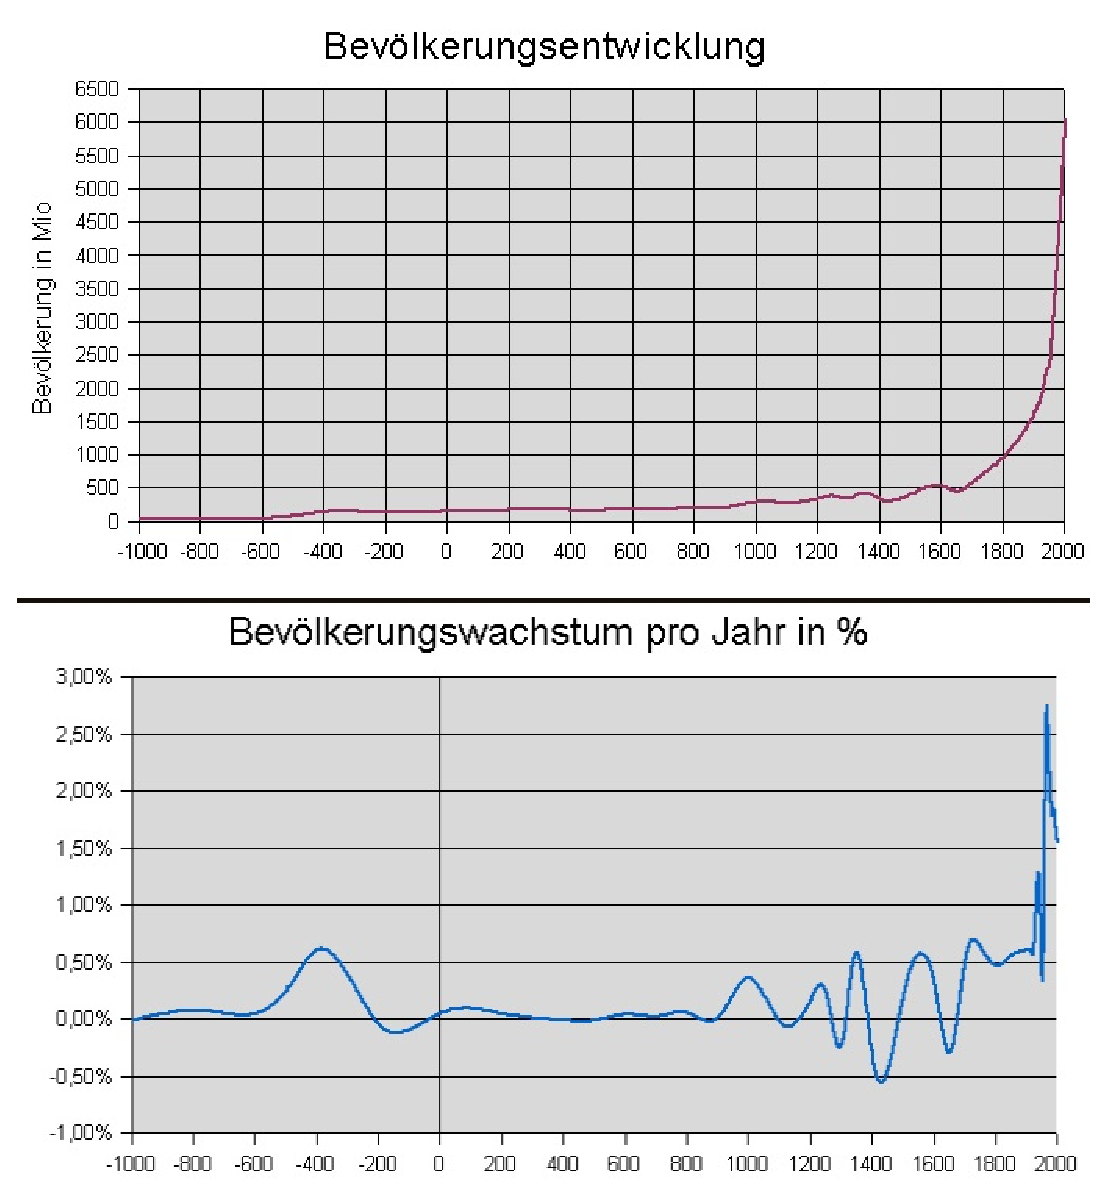
\includegraphics{../Bilder/Bild24-1.eps}}
				\begin{tiny}Quelle: https://upload.wikimedia.org/wikipedia/commons/8/8a/World-pop-hist-de-2.png\end{tiny}
								
				\begin{scriptsize}Abbildung 1\end{scriptsize}
				\end{center}
				
				\meinlr{\resizebox{1\linewidth}{!}{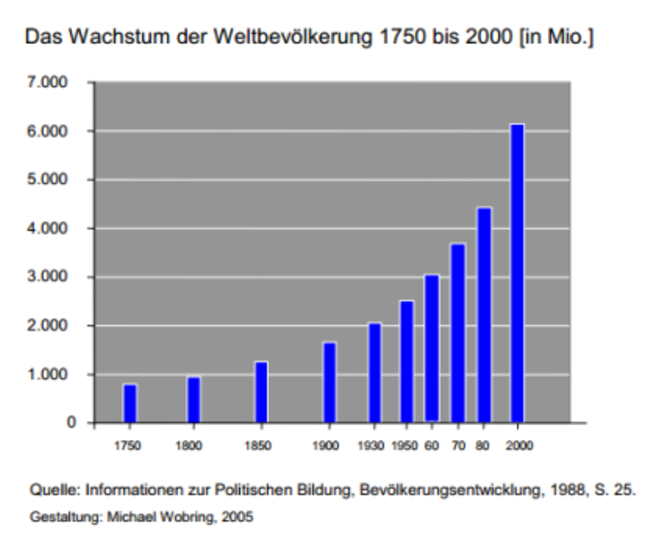
\includegraphics{../Bilder/Bild24-2.eps}}
								\begin{center}\begin{scriptsize}Abbildung 2\end{scriptsize}\end{center}}{\resizebox{1.4\linewidth}{!}{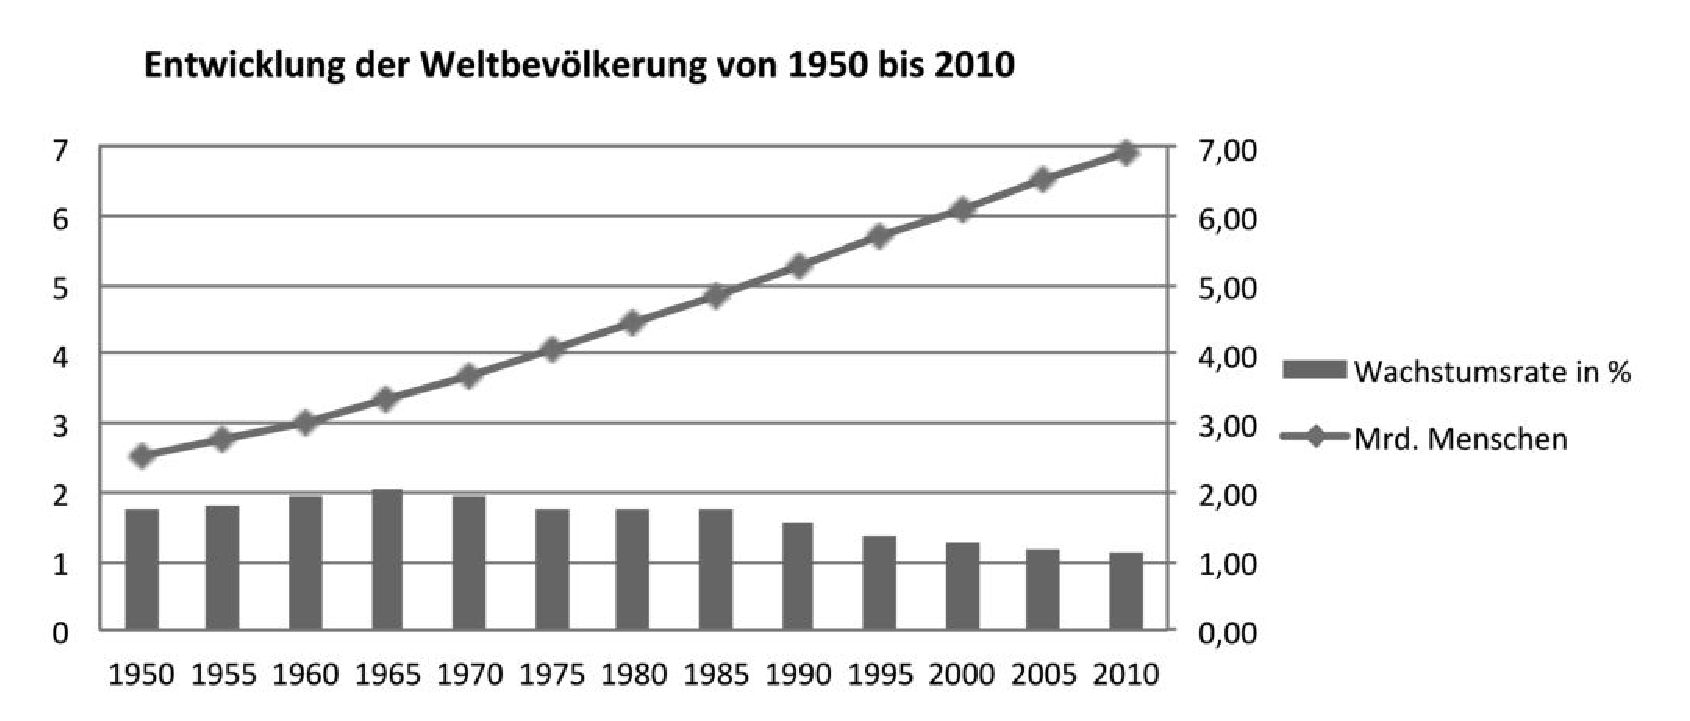
\includegraphics{../Bilder/Bild24-3.eps}}
								\begin{center}\begin{scriptsize}Abbildung 3\end{scriptsize}\end{center}}\leer
								
				\begin{scriptsize}				
				\begin{tabular}{|C{1.7cm}|C{1.7cm}|C{1.7cm}|C{1.7cm}|C{1.7cm}|C{1.7cm}|C{1.7cm}|}\hline
				Jahr&Afrika&Asien&Europa&Lateinamerika&Nordamerika&Ozeanien\\ \hline
				1900&133&925&430&74&82&6\\ \hline
				1950&227&1\,403&547&167&172&13\\ \hline
				1975&419&2\,379&676&323&242&21\\ \hline
				2000&819&3\,698&727&521&319&31\\ \hline				
				\end{tabular}
				\end{scriptsize}

\subsection{Aufgabenstellung:}
\begin{enumerate}
	\item Ermittle anhand der Abbildungen, um wie viele Menschen die Weltbev�lkerung von 1600 bis 18000 zugenommen hat!
	
	Nenne zwei Zeitr�ume, in denen die Weltbev�lkerung mindesten 100 Jahre lang abgenommen hat, und begr�nde ihre Antwort!
	
	\item Die Weltbev�lkerung hat von 1930 bis 1980 ann�hernd exponentiell zugenommen. Berechne unter dieser Annahme f�r diesen Zeitraum die j�hrliche Wachstumsrate auf Zehntelprozent genau!
	
	\item Begr�nde anhand der j�hrlichen Wachstumsraten aus Abbildung 3, warum die Entwicklung der Weltbev�lkerung von 1950 bis 2010 nicht durch eine Exponentialfunktion beschrieben werden kann!
	
Bei konstanter Zunahme der Bev�lkerungszahl ab 2010 wird f�r das Jahr 2050 eine Bev�lkerungszahl von 10,4 Milliarden prognostiziert.\\
Berechne, von welcher j�hrlichen Zunahme bei dieser Prognose ausgegangen wird!
Gib die j�hrliche Zunahme in Millionen Menschen an!

\item Angenommen, die absoluten Zahlen der Bev�lkerungsentwicklung der Kontinente und
Subkontinente im Zeitraum von 1900 bis 2000 werden in einem S�ulendiagramm mit
linearer Skalierung dargestellt.\\
Begr�nde, warum die starke Bev�lkerungszunahme in Ozeanien von 1900 bis 2000
in einem solchen Diagramm nicht erkennbar ist!

Gegeben sind f�nf Aussagen zur Bev�lkerungsentwicklung nach Kontinenten und Subkontinenten von 1900 bis 2000.\\
Kreuze die zutreffende(n) Aussage(n) an!\leer

\multiplechoice[5]{  %Anzahl der Antwortmoeglichkeiten, Standard: 5
				L1={Die Bev�lkerung Asiens hat sich im 20. Jahrhundert ann�hernd
vervierfacht.},   %1. Antwortmoeglichkeit 
				L2={Seit Beginn des 20. Jahrhunderts lebten in Lateinamerika mehr
Menschen als in Nordamerika.},   %2. Antwortmoeglichkeit
				L3={Im Zeitraum von 1975 bis 2000 war die relative Bev�lkerungszu-
nahme in Afrika am gr��ten.},   %3. Antwortmoeglichkeit
				L4={In Europa war die Bev�lkerungszunahme von 1975 bis 2000 ge-
ringer als von 1950 bis 1975.},   %4. Antwortmoeglichkeit
				L5={1950 lebten in Europa und Amerika zusammen bereits mehr als
eine Milliarde Menschen.},	 %5. Antwortmoeglichkeit
				L6={},	 %6. Antwortmoeglichkeit
				L7={},	 %7. Antwortmoeglichkeit
				L8={},	 %8. Antwortmoeglichkeit
				L9={},	 %9. Antwortmoeglichkeit
				%% LOESUNG: %%
				A1=1,  % 1. Antwort
				A2=3,	 % 2. Antwort
				A3=4,  % 3. Antwort
				A4=0,  % 4. Antwort
				A5=0,  % 5. Antwort
				}
						\end{enumerate}\leer
				
\antwort{\subsection{L�sungserwartung:}
\begin{enumerate}
	\item Zunahme von 1600 bis 1800: ca. 500 Millionen Menschen
	
	Die Weltbev�lkerung hat mindestens 100 Jahre lang abgenommen in [250 v. Chr.; 50 v. Chr.] (bzw. $[-250;-50]$) und $[1400;1500]$, da in diesen Zeitintervallen das j�hrliche Bev�lkerungswachstum in \% negativ ist.
	
	\item $N(t)=N_0\cdot a^t$\\
	$4,5=2\cdot a^50$\\
	$a\approx 1,016$, d.h. Zunahme um 1,6\,\% pro Jahr
	
	\item Bei einer exponentiellen Zunahme ist die j�hrliche Wachstumsrate konstant. Abbildung 3 zeigt, dass diese Voraussetzung im Zeitraum von 1950 bis 2010 nicht erf�llt ist.
	
	Konstante j�hrliche Zunahme von 2010 bis 2050:\\
	$\frac{10,4-6,9}{40}=0,0874$ Milliarden = 87,5 Millionen
	
	\item Da die Bev�lkerungszahl Ozeaniens von 1900 bis 2000 jeweils weniger als 1\,\% der
Bev�lkerungszahl Asiens betrug, sind die entsprechenden S�ulen f�r Ozeanien sehr
niedrig (H�he fast null).\\
Daher ist die Verf�nffachung der Bev�lkerungszahl Ozeaniens nicht erkennbar.

L�sung Multiple Choice siehe oben
			\end{enumerate}}
		\end{langesbeispiel}